\documentclass[extendedabs]{recpad2k}

% Caption formatting to match the Word template
\usepackage[font={footnotesize,color=captionblue},labelfont=normalfont,textfont=normalfont,skip=4pt,justification=centering,belowskip=0pt]{caption}


\setlength{\floatsep}{4pt plus 1pt minus 1pt}
\setlength{\textfloatsep}{4pt plus 1pt minus 1pt}
\setlength{\intextsep}{4pt plus 1pt minus 1pt}
\setlength{\abovecaptionskip}{3pt}
\setlength{\belowcaptionskip}{0pt}
\definecolor{captionblue}{RGB}{0,26,102}

\usepackage{booktabs}
\usepackage{float}
\usepackage{balance}
\usepackage{placeins}
\usepackage{xcolor}
\usepackage[normalem]{ulem} % Provides \sout while 

% Permit line breaks after underscores inside model identifiers
\newcommand{\ubk}{\_\allowbreak}
\newcommand{\cut}[1]{{\color{red}\sout{#1}}}
\newcommand{\add}[1]{{\color{green!50!black}#1}}
% Last-resort stretch so long identifiers never overrun the narrow columns
\setlength{\emergencystretch}{2em}

% Fitting: heading space trimmed from the class defaults (-12pt/6pt) over six
% headings. Revert these two lines to restore the template spacing exactly.
\makeatletter
\renewcommand\section{\@startsection{section}{1}{\z@}%
  {-12pt}{6pt}%
  {\normalfont\normalsize\bfseries\sffamily\flushleft\textcolor{bmv@sectioncolor}}}
\makeatother

\title{Prompted Large Language Models for Narrative Participant\\Extraction in Parallel Portuguese and English News}

\addauthor{Davi Santos}{davibarrel98@gmail.com}{1}
\addauthor{Evelin Amorim}{evelin.f.amorim@inesctec.pt}{1}
\addauthor{Alípio Jorge}{amjorge@fc.up.pt}{1}

\addinstitution{
 Faculdade de Ci\^encias\\
 Universidade do Porto\\
 Porto, Portugal
}

\runninghead{Santos, Amorim, Jorge}{Prompted LLMs for Participant Extraction}

\def\eg{\emph{e.g}\bmvaOneDot}
\def\etal{\emph{et al}\bmvaOneDot}
\def\ie{\emph{i.e}\bmvaOneDot}

\begin{document}

\maketitle

\begin{abstract}
Narrative Extraction turns unstructured news into structured records of the events a story reports, and participants are the named entities on which those events depend. Existing work either supplies the participant spans or compares the two languages over separate corpora, so neither the joint recovery of a span and its semantic type nor the effect of the language has been measured under controlled conditions. This work evaluates nine prompted large language models, seven open and of 4B to 14B parameters, on that joint task over 117 news articles in parallel Portuguese and English versions, across eight prompt variants, three decoding temperatures and two query granularities. Prompt composition and query granularity govern the outcome while the language does not, and the ceiling sits at span identification rather than attribute assignment.
\end{abstract}
%-------------------------------------------------------------------------

\section{Introduction}
\label{sec:intro}

Narratives are sequences of linked events involving elements such as organizations, people, times and locations, and Narrative Extraction applies computational tools to identifying them~\cite{Santanaetal2023}. Among these, participants constitute the ``who'' that grounds the ``what'' of a story~\cite{Text2StoryLusa}: a participant is a named entity that plays a role in the events and carries a semantic type, such as person, organization or location. Recovering them supports entity-centred summarization and storyline tracking.

Participant recognition in Portuguese is constrained by scarce schema-specific training data: supervised token classification depends on large annotated corpora~\cite{santos2023dip}, and unsupervised entity linking over Portuguese news reaches about 0.40 F1~\cite{machado2024identification}. Prompted decoder models need no annotated corpus and approach encoder results once the prompt carries an entity definition and a solved example~\cite{Sousaetal2023,hu2024improving}, which makes prompt design a methodological variable. Whether their bottleneck lies in span-boundary detection or in attribute classification remains open, as does their relative performance in Portuguese and English given the resource imbalance between the two~\cite{Almeida2023}.

This work examines prompted participant extraction as a method rather than searching for its best configuration, on a corpus whose articles are annotated in both languages~\cite{Text2StoryLusa}, so content stays constant while the language changes. It assesses how prompt sensitivity varies across languages and between span detection and attribute classification, whether errors are shared across the parallel versions, whether the ceiling lies in span identification or attribute assignment, and whether cross-lingual assistance, \ie extracting from the English translation of a Portuguese article (translate-test), mitigates these limitations. It contributes a bilingual benchmark of nine models, a joint span-and-type evaluation under strict and relaxed criteria, and a sentence-level decomposition that localizes the bottleneck.

%-------------------------------------------------------------------------
\section{Methods}
\label{sec:method}

\begin{table}[!t]
\centering
\captionsetup{position=bottom}
{\scriptsize
\begin{tabular}{@{}l ccc@{}}
\toprule
\textbf{Language} & \textbf{Docs} & \textbf{Participants} & \textbf{Tokens/doc} \\
\midrule
Portuguese & 117 & 3530 & $155.1 \pm 28.9$ \\
English    & 116 & 3502 & $152.5 \pm 29.4$ \\
\bottomrule
\end{tabular}}
\caption{Corpus summary per language. Tokens are whitespace-delimited over the full article text.}
\label{tab:corpus}
\end{table}


\noindent\textbf{Dataset.} The Lusa Annotated Dataset~\cite{Text2StoryLusa} holds 117 European Portuguese news articles annotated with narrative elements, 116 with a parallel English version automatically translated with the Google Translate API\footnote{\url{https://docs.cloud.google.com/translate/docs/reference/rest}} and aligned with LinguAligner\footnote{\url{https://github.com/lfcc1/LinguAligner}}. One instance serves as the one-shot demonstration, 19 form the prompt-selection partition and the remaining 97 (PT) and 96 (EN) the test partition, with 2580 annotated participants each. Only participant annotations are used. A participant is annotated as the full noun phrase that refers to it, leading article or contraction included (\emph{a ex-companheira}, ``the ex-partner''), so 60.3\% (PT) and 49.4\% (EN) of annotated test spans open with a determiner. Each carries one of nine semantic types, skewed and near-identical across languages: person, organization and location cover 74\% of participants in both.

\noindent\textbf{Prompt design.} The experiment adopts the prompts of Sousa \etal~\cite{Sousaetal2023}. All are written in English regardless of article language and combine three components in fixed order: a task description asking for participant spans (\texttt{ext}) or spans with their types (\texttt{cls}), an optional definition of narrative participant (\texttt{def}), and an optional one-shot solved example in the article's language (\texttt{exp}). The eight variants, from the bare \texttt{ext} to \texttt{cls\ubk{}def\ubk{}exp}, form the complete $2\times2\times2$ design over task framing (\texttt{ext}/\texttt{cls}), definition and example, so the effect of each component is measured with the other two held fixed.

\noindent\textbf{Models and regimes.} Nine models are evaluated on a pipeline extending that of Sousa \etal~\cite{Sousaetal2023}: \texttt{gemma3\ubk{}4b}, \texttt{gemma3\ubk{}12b}, \texttt{qwen3\ubk{}4b}, \texttt{qwen3\ubk{}8b} and \texttt{qwen3\ubk{}14b}, from two well-studied open-weight families whose sizes pair across them (4B with 4B, 12B with 14B), to vary scale within and across families; the European Portuguese \texttt{gervasio\ubk{}8b\ubk{}ptpt} and \texttt{amalia} and the multilingual European \texttt{euro\ubk{}llm\ubk{}9b}, to test language specialisation; and \texttt{gemini}~2.5~Flash as a proprietary upper reference. Open models are capped at 14B parameters by the compute available on the Deucalion supercomputer. The document-level regime submits each article in one query: a selection phase scores the eight variants over 19 articles per language at temperature 0.3, and a test phase applies the best variant by F1-ext to the held-out articles at 0.3, 0.6 and 1. The sentence-level regime submits one sentence at a time to \texttt{qwen3\ubk{}14b} at 0.3, in the consecutive stages of detection, extraction and classification.

\noindent\textbf{Evaluation.} The strict F1-ext credits a prediction only when its span coincides exactly with an annotated one, so a single missing word counts as both a false positive and a false negative; typing accuracy is the share of exactly matched spans whose type is also correct. F1-ext pools its counts over the corpus and is therefore micro-averaged. The relaxed F1-r aligns each predicted span, word by word, with the annotation sharing the most words via the Ratcliff/Obershelp algorithm~\cite{ratcliff1988pattern}; aligned words are true positives, unaligned predicted words false positives and unaligned annotated words false negatives. It is computed per document and averaged over documents, and is therefore macro-averaged.

%-------------------------------------------------------------------------
\section{Results and Discussion}
\label{sec:results}

\begin{figure}[!ht]
\centering
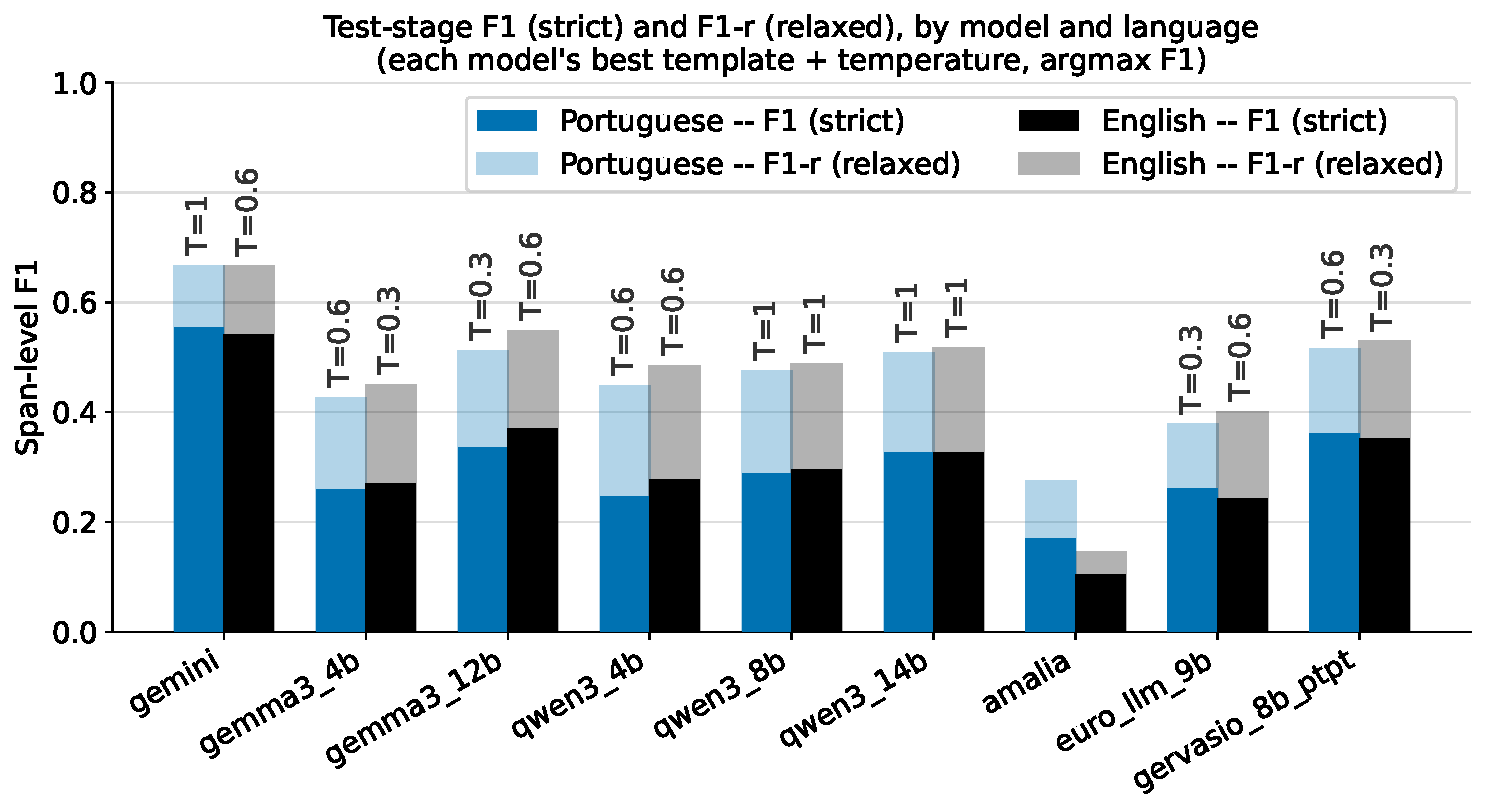
\includegraphics[width=0.72\linewidth,trim=0 0 0 50,clip]{figures/02_f1_f1r_leaderboard.pdf}
\caption{Test-phase strict span-level F1 (F1-ext, solid fill) and relaxed word-level F1 (F1-r, full bar) per model and language, at the best prompt variant and temperature $T$ (bar labels).}
\label{fig:leaderboard}
\end{figure}

Of the 8015 document-level answers over both phases, languages and temperatures, 98.0\% were parsed; abstentions (1.8\%) concentrate in \texttt{amalia}, which refused articles on sensitive topics such as crime and murder. Figure~\ref{fig:leaderboard} gives the test-phase picture. The baseline \texttt{gemini} leads both criteria in both languages and no open model reaches it. Except for \texttt{amalia}, each model scores similarly in both languages and the ranking is largely unchanged.

The prompt governs span extraction far more than the language or the temperature does. Over the nine models, the median selection-phase F1-ext rises from 0.078 (bare \texttt{ext}) to 0.226 (\texttt{cls\ubk{}def\ubk{}exp}) in Portuguese and from 0.080 to 0.292 in English; the four variants carrying the one-shot example occupy the four highest ranks in both languages and the four without it the four lowest, without exception. The gain is in recall: the example does not sharpen the predictions a model already makes but leads it to extract more of the annotated participants. On an article reporting that a man shot his former partner, \texttt{qwen3\ubk{}14b} under \texttt{ext} outputs only ``Homem'' and ``Ex-companheira''; under \texttt{ext\ubk{}exp} it adds exact matches such as ``Um homem'', ``a mulher'', ``Grijó'' and ``Vila Nova de Gaia'', yet outputs ``Polícia Judiciária'' and ``ex-companheira'' where the annotation holds ``a Polícia Judiciária'' and ``a ex-companheira'' meaning partial matches. The example thus conveys what counts as a participant but only partly where its span begins, a convention \texttt{gemini} adopts and the open models largely do not. The definition is the weaker component. Prompt sensitivity, the standard deviation of F1-ext over the eight variants, differs across models but not across languages, and typing accuracy stays above 0.70 across the four \texttt{cls\ubk{}*} variants.

\begin{table}[H]
\centering
\captionsetup{position=bottom}
{\scriptsize
\setlength{\tabcolsep}{2pt}
\begin{tabular}{@{}l rrrr rrrr@{}}
\toprule
& \multicolumn{4}{c}{\textbf{Portuguese}} & \multicolumn{4}{c}{\textbf{English}} \\
\cmidrule(lr){2-5}\cmidrule(l){6-9}
\textbf{Model} & \textbf{F1-ext} & \textbf{Loc.} & \textbf{Typed} & \textbf{Acc.} & \textbf{F1-ext} & \textbf{Loc.} & \textbf{Typed} & \textbf{Acc.} \\
\midrule
\texttt{gemini}                & 0.553 & 1434 & 1279 & 0.892 & 0.542 & 1414 & 1224 & 0.866 \\
\texttt{gemma3\ubk{}4b}        & 0.258 & 542  & 446  & 0.823 & 0.270 & 576  & 479  & 0.832 \\
\texttt{gemma3\ubk{}12b}       & 0.335 & 772  & 640  & 0.829 & 0.370 & 875  & 718  & 0.821 \\
\texttt{qwen3\ubk{}4b}         & 0.246 & 554  & 464  & 0.838 & 0.277 & 719  & 575  & 0.800 \\
\texttt{amalia}                & 0.169 & 361  & 285  & 0.789 & 0.105 & 195  & 148  & 0.759 \\
\texttt{euro\ubk{}llm\ubk{}9b} & 0.260 & 565  & 433  & 0.766 & 0.242 & 591  & 412  & 0.697 \\
\texttt{qwen3\ubk{}14b} (sent.) & 0.451 & 1031 & 927 & 0.899 & 0.430 & 999  & 883  & 0.884 \\
\bottomrule
\end{tabular}}
\caption{Test-phase runs that return types, out of 2580 annotated participants per language. \textbf{F1-ext}: strict span-level F1; \textbf{Loc.}: located, \ie exact span matches; \textbf{Typed}: located and correctly typed; \textbf{Acc.}: typing accuracy, Typed/Loc. Document-level runs at the best temperature, the sentence-level run (sent.) at $T=0.3$; only models whose selected variant requests types (\texttt{cls\_*}) appear.}
\label{tab:funnel}
\end{table}

Table~\ref{tab:funnel} locates the ceiling: in every run more participants are missed at span identification than are mistyped after being located, and the strongest run identifies 1434 of the 2580 annotated Portuguese participants and types 1279 of them correctly. The sentence-level regime confirms this by recording each stage: detection retains 84.9\%--93.5\% of sentences containing an annotated participant and classification types 86.2\%--89.9\% of the spans it receives, while extraction recovers fewer than half of the participants passed to it.

Partial matches explain the gap between F1-ext and F1-r: in both languages the errors concentrate on the first word of a span. Figure~\ref{fig:wordpos2} illustrates this pattern for two-word participants not recovered exactly, which account for about 40\% of partial matches. Their first-word match rates are 14\% (PT) and 30\% (EN), compared with 68\% and 61\%, respectively, for the second word; articles and determiners account for 75\% (PT) and 63\% (EN) of first-word errors. Longer participants show the same pattern at both granularities. The models thus identify the correct entity but omit its leading determiner. A deterministic rule that prepends the word preceding each predicted span whenever it is an article or contraction raises the median F1-ext of the nine document-level runs at $T=0.3$ from 0.260 to 0.323 (PT) and from 0.287 to 0.388 (EN); crediting every span one leading function word away from a missed annotation bounds the gain at 0.471 and 0.468. It lowers \texttt{gemini} (0.506 to 0.478, PT), which already includes the determiner, so the convention is better conveyed to the model than imposed afterwards.

Translate-test therefore offers little benefit, and neither language is consistently better: in Table~\ref{tab:funnel} four runs favour Portuguese and three English, by no more than separates two temperatures of the same model. A plausible reason is that the models recognise the entity in either language but not the boundary convention of the annotation scheme, such as whether the leading article belongs to the span; this convention is specific to the schema rather than to the language, so translation leaves it unchanged. Input granularity matters more: at sentence level \texttt{qwen3\ubk{}14b} rises from 0.313 to 0.451 (PT) and 0.312 to 0.430 (EN).

\begin{figure}[!h]
\centering
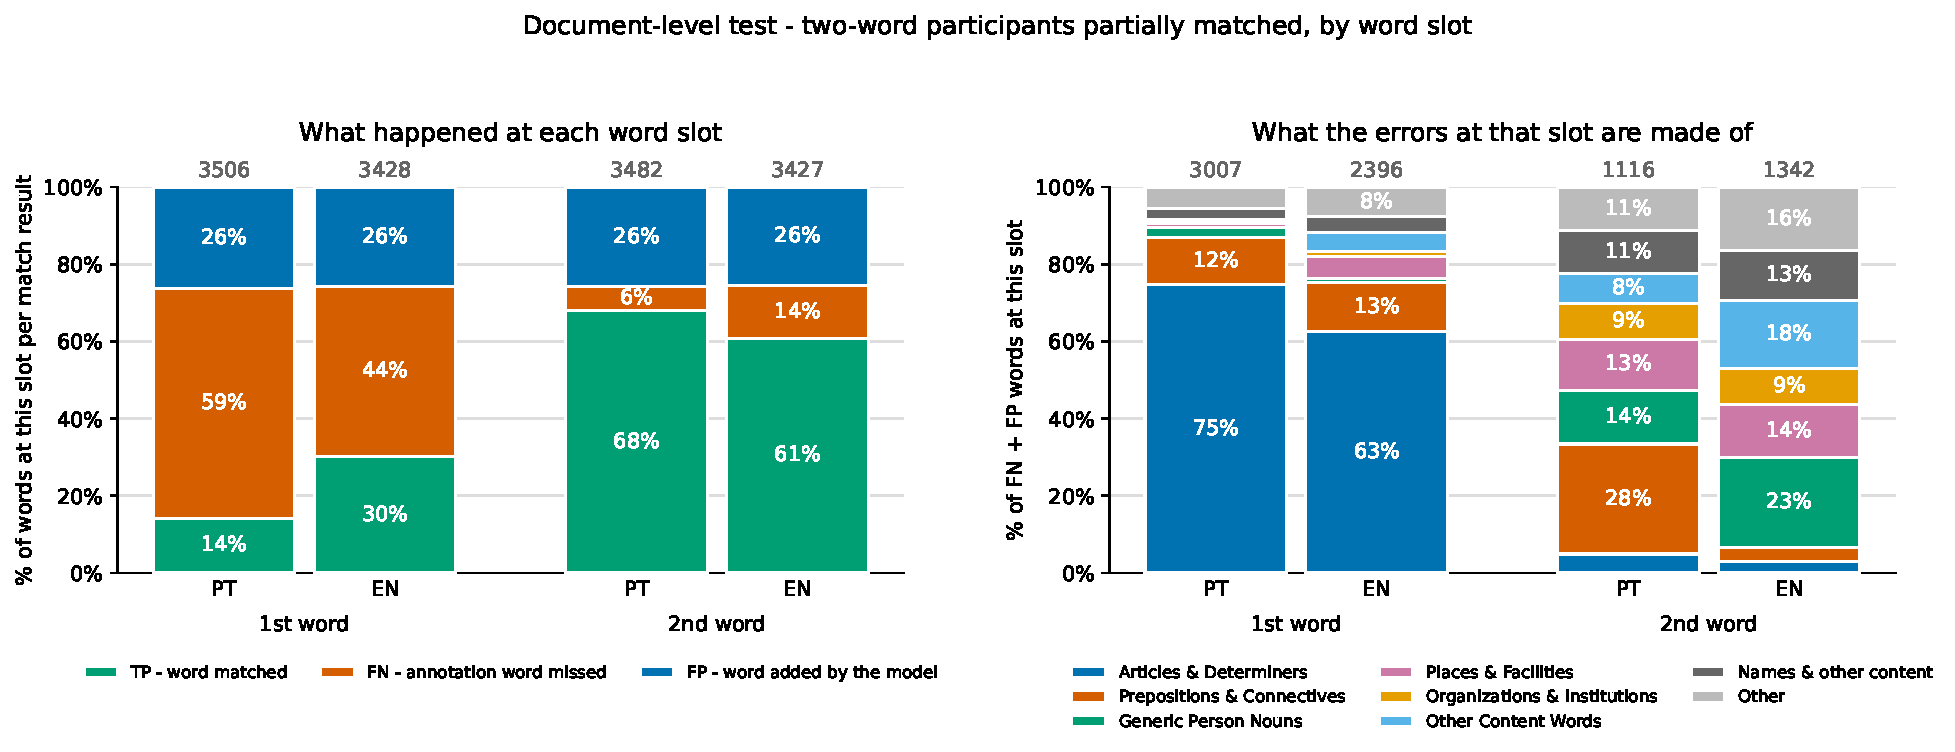
\includegraphics[width=0.70\linewidth,trim=0 0 480 40,clip]{figures/09_word_position_len2_test.pdf}
\caption{Outcome of each word of two-word annotated participants matched only partially (document-level test phase, pooled over models). TP: word matched; FN: annotated word missed; FP: word added. Numbers above bars are word counts.}
\label{fig:wordpos2}
\end{figure}

%-------------------------------------------------------------------------
\FloatBarrier
\section{Final Remarks and Next Steps}
\label{sec:conclusions}
\balance

The ceiling of the joint task sits at span identification rather than attribute assignment: typing accuracy stays between 0.70 and 0.90, while the strongest run recovers 1434 of 2580 participants. The one-shot example and single-sentence input each move strict extraction further than any temperature or language does, and the errors, shared between languages and concentrated on the leading determiner, place the limitation in the method rather than in the language. Future work should target this boundary error with a guideline prompt in the style of LiP-NER~\cite{lipner2025}, stating the scheme's convention as a literal rule, \ie that a participant span opens with its article or contraction (``a'', ``o'', ``na'', ``do''; ``the'', ``a''), and pairing it with demonstrations that keep the determiner. The sentence-level decomposition should also be extended to other models.

% %-------------------------------------------------------------------------
\textbf{Acknowledgments}. Funded by FCT I.P. (doi:10.54499/\allowbreak UID/\allowbreak 50014/2025) and, on Deucalion, by EuroHPC JU and Portugal (2026.00026.\allowbreak AIVLAB.\allowbreak DEUCALION).
% This work uses the Lusa Annotated Dataset produced within the Text2Story project, and was supported by .

{\scriptsize
\bibliography{refs}
}

\end{document}
